\documentclass{ximera}

% MATH -----------------------------------------------------------
\newcommand{\nats}{\mathbb N}
\newcommand{\ints}{\mathbb Z}
\newcommand{\rats}{\mathbb Q}
\newcommand{\reals}{\mathbb R}
\newcommand{\complex}{\mathbb C}
\newcommand{\powerset}{\mathscr P}

%-------------------------------------------------------------

\pgfplotsset{compat=1.18}
\begin{document}
\begin{abstract}
 \end{abstract}

    \title{Exemplar Examples 2}
    
    \maketitle

Let's consider the first order separable differential equation $y^{\,\prime}=2xe^y$.

% y=-ln(1-x^2) for x in (-1,1).  y'=2x/(1-x^2)=2xe^y

\begin{enumerate}

\item Here is an (approximate) direction field for this differential equation on \\$[-2,2]\times [-2,2]$.  Let's draw (part of) the solution curve to this differential equation that passes through the point $(0,0)$.  Let's use our drawing to estimate the value of this solution when $x=0.5$.\\
\begin{figure}[h]
\centering
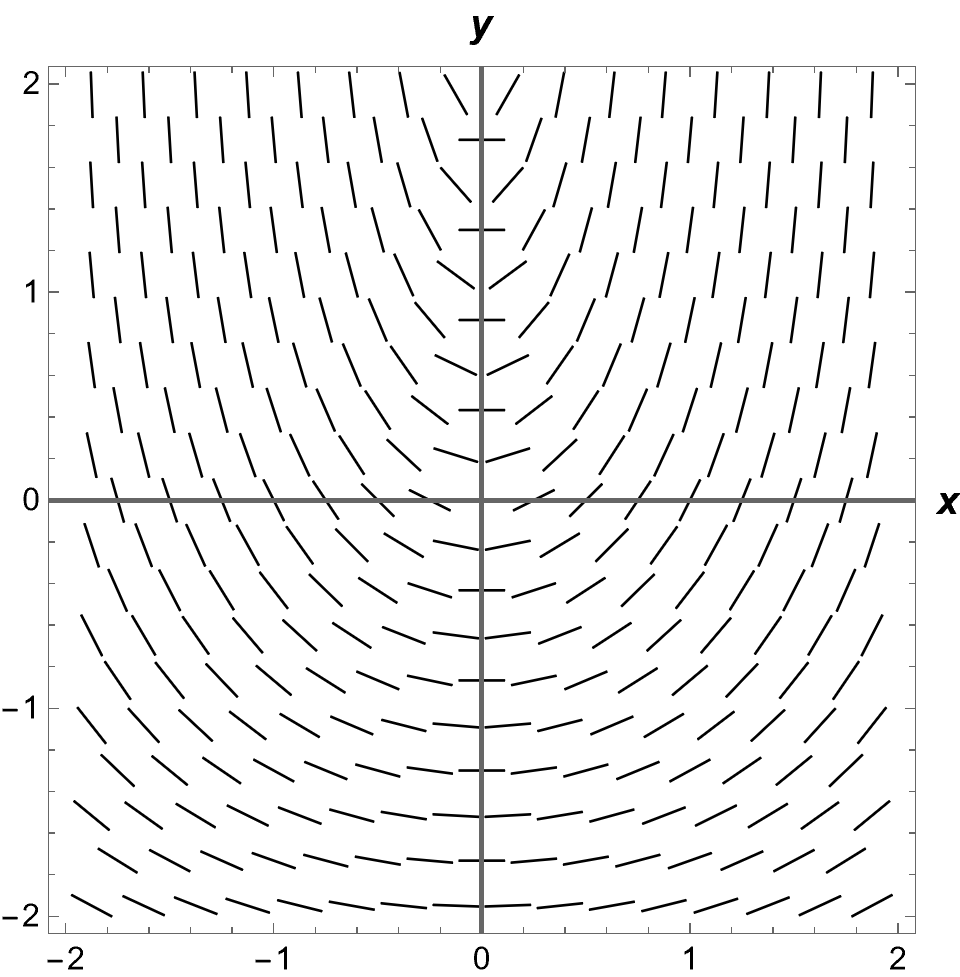
\includegraphics[scale=0.6,alt={A direction field.}]{ExemplarTwoDirectionField.png}
\caption{A direction field}
\end{figure}

% About 0.2

\item Does this equation have any constant solutions?\\ \\

% NO!

\item Let's write this equation the form $h(y)y^{\,\prime}=g(x)$.  

\vfill

% e^(-y)y'=2x

\item Let's integrate both sides with respect to $x$.

% -e^(-y)=x^2+C  -

\vfill

\newpage


\item Now let's solve this differential equation for its general solution, and determine the solution that passes through $(0,0)$.

% -y=ln|-x^2+C|  -

% y=-ln|-x^2+C|=ln|1/(C-x^2)|.  C=1.  y=-ln|1-x^2|


\vfill

\vfill

\vfill
\item  How good was our estimate?

\vfill

\item Let's determine the interval $I$ such that our solution is valid on $I$, but not valid on any interval $J\neq I$ that contains $I$. 

% (-1,1)

\vfill

\vfill

\end{enumerate}


\end{document}